\section{Classes} \label{sc:classes}
Based on the initial interviews and ongoing communication with the representatives from Aalborg Zoo, a class diagram has been constructed (figure \ref{fig:FirstPDClassDiagram}). In this diagram the different classes are illustates along with the relations between them. 
%This understanding has been achieved through the initial interviews and ongoing communication with the representatives from Aalborg Zoo. Below is a class diagram illustrating the different classes and their relations (\autoref{fig:FirstPDClassDiagram}), followed by further explanations of the different classes and these relations.

% Figur af klassediagrammet
\begin{figure}[H]
    \centering
    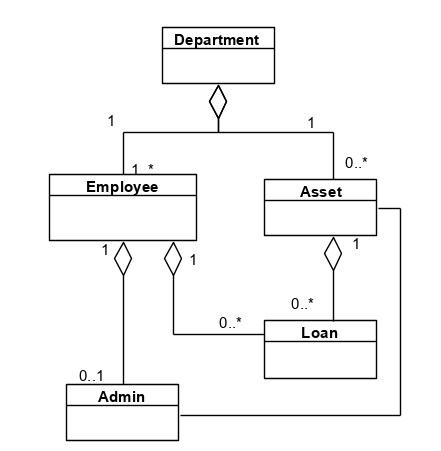
\includegraphics[width=1.0\textwidth]{figures/PDDiagramV4.png}
    \caption{Class diagram of the immediate classes in the problem domain.}
    \label{fig:FirstPDClassDiagram}
\end{figure}

% Beskriv den overordnede ide med systemet ud fra klassediagrammet

\textbf{Department}\\
A department is a division of the employees and assets at the zoo.

\todo{Insert following comment to implementation description of department}
% The department class represents the departments at the zoo. Unlike the way a department is understood in the problem domain and is structure in the real world, a department in the system has assets and tags. The users can then search within the different departments to find a given asset. The departments then function as further division for both tags and assets, to give a simpler overview of both for a user from a specific department. This hinders a flood of irrelevant assets and tags related to other departments when, as an example, the IT department wants to find one of their assets. The way departments and users are related in this construction is only as a user has a standard department, with which they are presented with as they launch the application. They can change department to search for assets in departments other than their own.

\textbf{Asset}\\
An instance of the asset class is an asset being kept track of in the problem domain. Assets belong to a department and can be loaned out to employees.
\par

\textbf{Employee} \\
An employee is part of a department and can borrow assets. Some employees also have the role of Admin.
\par

\textbf{Admin} \\
An admin has a relation to assets, which he can loan out to other employees.
\par
Now that the main classes in the problem domain and their relations have been defined and depicted, explaining and depicting their states through the systems life-cycle is the next step to adequately represent the problem domain.

